%%%%%%%%%%%%%%%%%%%%%%%%%%%%%%%%%%%%%%%%%
% Beamer Presentation
% LaTeX Template
% Version 1.0 (10/11/12)
%
% This template has been downloaded from:
% http://www.LaTeXTemplates.com
%
% License:
% CC BY-NC-SA 3.0 (http://creativecommons.org/licenses/by-nc-sa/3.0/)
%
%%%%%%%%%%%%%%%%%%%%%%%%%%%%%%%%%%%%%%%%%

%----------------------------------------------------------------------------------------
%	PACKAGES AND THEMES
%----------------------------------------------------------------------------------------

\documentclass{beamer}

\mode<presentation> {

% The Beamer class comes with a number of default slide themes
% which change the colors and layouts of slides. Below this is a list
% of all the themes, uncomment each in turn to see what they look like.

%\usetheme{default}
%\usetheme{AnnArbor}
%\usetheme{Antibes}
%\usetheme{Bergen}
%\usetheme{Berkeley}
%\usetheme{Berlin}
%\usetheme{Boadilla}
%\usetheme{CambridgeUS}
%\usetheme{Copenhagen}
%\usetheme{Darmstadt}
%\usetheme{Dresden}
%\usetheme{Frankfurt}
%\usetheme{Goettingen}
%\usetheme{Hannover}
%\usetheme{Ilmenau}
%\usetheme{JuanLesPins}
%\usetheme{Luebeck}
%\usetheme{Madrid}
%\usetheme{Malmoe}
%\usetheme{Marburg}
%\usetheme{Montpellier}
%\usetheme{PaloAlto}
%\usetheme{Pittsburgh}
%\usetheme{Rochester}
%\usetheme{Singapore}
%\usetheme{Szeged}
\usetheme{Warsaw}

% As well as themes, the Beamer class has a number of color themes
% for any slide theme. Uncomment each of these in turn to see how it
% changes the colors of your current slide theme.

%\usecolortheme{albatross}
%\usecolortheme{beaver}
%\usecolortheme{beetle}
%\usecolortheme{crane}
%\usecolortheme{dolphin}
%\usecolortheme{dove}
%\usecolortheme{fly}
%\usecolortheme{lily}
%\usecolortheme{orchid}
%\usecolortheme{rose}
%\usecolortheme{seagull}
%\usecolortheme{seahorse}
%\usecolortheme{whale}
%\usecolortheme{wolverine}

%\setbeamertemplate{footline} % To remove the footer line in all slides uncomment this line
%\setbeamertemplate{footline}[page number] % To replace the footer line in all slides with a simple slide count uncomment this line

%\setbeamertemplate{navigation symbols}{} % To remove the navigation symbols from the bottom of all slides uncomment this line
}

\usepackage{graphicx} % Allows including images
\usepackage{booktabs} % Allows the use of \toprule, \midrule and \bottomrule in tables
\usepackage{listings}
\usepackage{color}
\usepackage{hyperref}
\usepackage[lofdepth,lotdepth]{subfig}

\definecolor{codegreen}{rgb}{0,0.6,0}
\definecolor{codegray}{rgb}{0.5,0.5,0.5}
\definecolor{codepurple}{rgb}{0.58,0,0.82}
\definecolor{backcolour}{rgb}{0.95,0.95,0.92}

\lstdefinestyle{mystyle}{
    backgroundcolor=\color{backcolour},   
    commentstyle=\color{codegreen},
    keywordstyle=\color{magenta},
    numberstyle=\tiny\color{codegray},
    stringstyle=\color{codepurple},
    %basicstyle=\footnotesize,
    basicstyle=\scriptsize\ttfamily,
    breakatwhitespace=false,         
    breaklines=true,                 
    captionpos=b,                    
    keepspaces=true,                 
    numbers=left,                    
    numbersep=5pt,                  
    showspaces=false,                
    showstringspaces=false,
    showtabs=false,                  
    tabsize=2,
    language=bash
}
 
\lstset{style=mystyle}

%----------------------------------------------------------------------------------------
%	TITLE PAGE
%----------------------------------------------------------------------------------------

\title[Introduction to GitFlow]{Introduction to GitFlow} % The short title appears at the bottom of every slide, the full title is only on the title page

\author{Nicolas Barrier} % Your name
\institute[UMR MARBEC] % 
{
UMR MARBEC \\ % Your institution for the title page
\medskip
\textit{nicolas.barrier@ird.fr} % Your email address
}
\date{\today} % Date, can be changed to a custom date

\begin{document}

\begin{frame}
\titlepage % Print the title page as the first slide
\begin{center}

\includegraphics[height=2cm]{logo-marbec.png}
\hspace{1em}

\includegraphics[height=2cm]{logo_ird.png}
\end{center}
\end{frame}

\begin{frame}
\frametitle{Introduction} % Table of contents slide, comment this block out to remove it
There are several ways to use GIT (we talk about \textbf{workflows}). 

\begin{itemize}
    \item \emph{Centralized workflow}: one main branch, everyone commit in the same place.
    \item \emph{Feature Branch Workflow}: developments are made in dedicated branches (feature branches), which are regularly merged to the master one.
    \item \textbf{\textit{Gitflow Workflow}}: Strict branching model designed around the project release.
\end{itemize}

Source: \url{https://www.atlassian.com/git/tutorials/comparing-workflows}) for more details.

\end{frame}

\begin{frame}{GitFlow branches}

GitFlow workflow contains two main branches:
\begin{itemize}
\item{\emph{master:} official release history. Branch which is shared to the world!}
\item{\emph{develop:} integration branch for features}
\end{itemize}

It also contains additional temporal branches:
\begin{itemize}
\item{\emph{feature}: feature branches (one for each new feature to add to the code)}
\item{\emph{release}: branch created when enough features have been added (new version of the code)}
\item{\emph{hotfix}: branch for maintenance and bug correction of the production release}
\end{itemize}

\end{frame}

\begin{frame}{In summary...}

\begin{center}
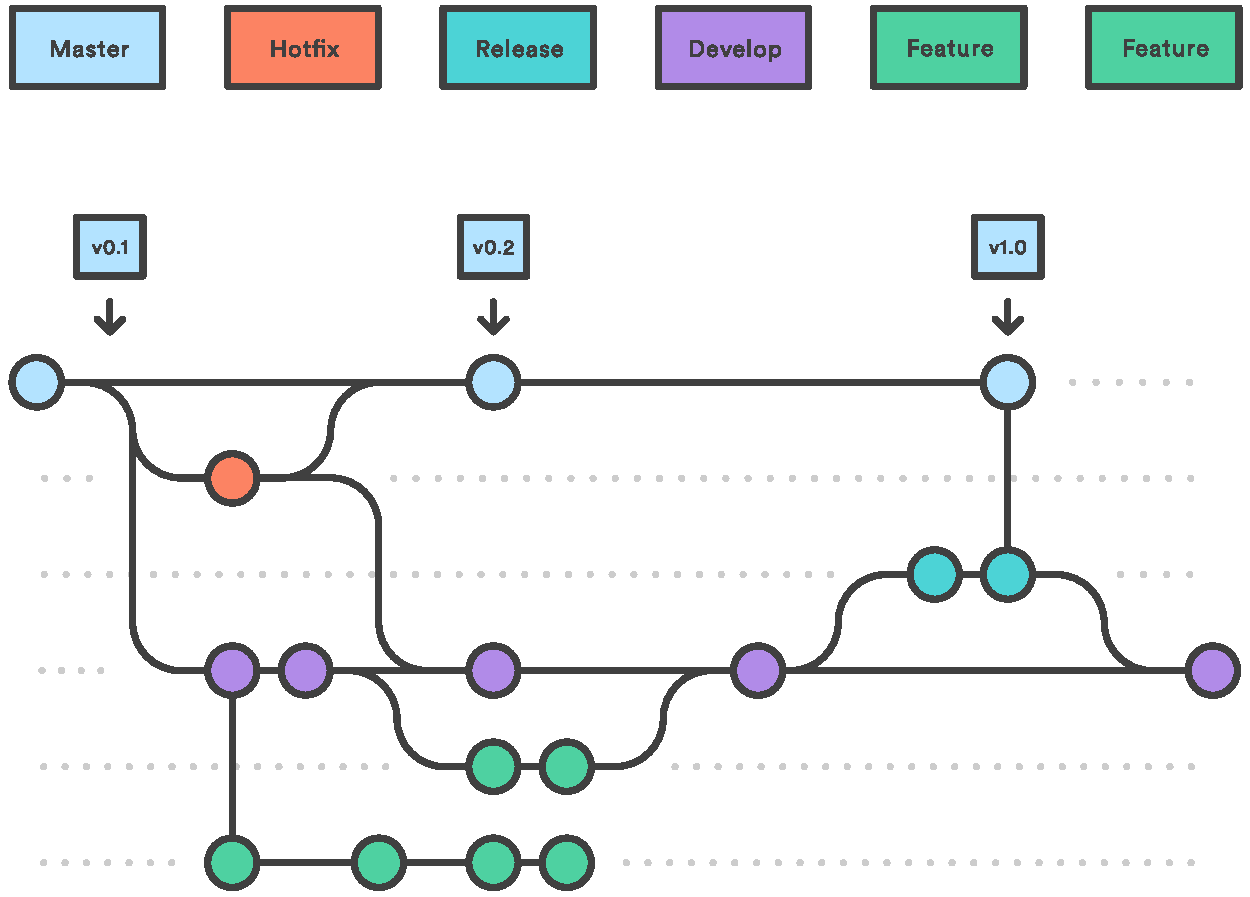
\includegraphics[scale=0.5]{05-_2_.pdf}    
\end{center}

\end{frame}    

\begin{frame}[fragile]{How it works in practice}

Install the GitFlow extension:

\begin{lstlisting}[language=bash]
sudo apt-get install git-flow
\end{lstlisting}

\vspace{1em}
Now, from your directory, initialize the GitFlow workflow:

\begin{lstlisting}[language=bash]
git flow init # create the develop branch
git push origin develop # push the develop branch to the repository
\end{lstlisting}

\end{frame}

\begin{frame}[fragile]{Creating new features}

\begin{lstlisting}
# recovers the latest develop branch
git pull origin develop

# create feature branch from develop and switch to it
git flow feature start my-feature 

# put the feature branch to the repo (not necessary)
git flow feature publish my-feature 

# edit/add files: new functionalities

# commit changes to the my-feature branch
git commit 

# merge my-feature branch with develop and remove it
# switch back to develop
git flow feature finish

# push updated develop branch
git push origin develop

# if conflict (someone has already pushed in develop)
git pull origin develop
git push origin develop
\end{lstlisting}

\end{frame}

\begin{frame}[fragile]{Creating a new release}

\begin{lstlisting}
# recovers the latest develop branch
git pull origin develop

# create a new release branch
git flow release start my-release

# put the release branch to the repo (not necessary)
git flow release publish my-release 

# edit/add files: bug fixes + documentation

# commit changes to the my-feature branch
git commit 

# finish the release
git flow release finish

# push updated develop/master and tags
git push origin --tags
git push origin develop
git push origin master
\end{lstlisting}
\end{frame}

\begin{frame}[fragile]
\frametitle{Creating hotfixes}
\begin{lstlisting}
# recovers the latest develop/master branches
git pull origin develop

# create a new hotfix branch from master
# name should be a version name (1.3.2 for instance)
git flow hotfix start hotfix-tag

# edit/add files: bug corrections

# commit changes to the hotfix-tag branch
git commit 

# finish the release
# merge hotfix branch to master/develop
git flow hotfix finish

# push updated develop/master and tags
git push origin --tags
git push origin develop
git push origin master
\end{lstlisting}
\end{frame}

\begin{frame}
\frametitle{References} % Table of contents slide, comment this block out to remove it

\begin{itemize}
    \item \url{https://nvie.com/posts/a-successful-git-branching-model/}
    \item \url{https://www.atlassian.com/git/tutorials/comparing-workflows}
    \item \url{https://danielkummer.github.io/git-flow-cheatsheet/}
    \item \url{https://gist.github.com/JamesMGreene/cdd0ac49f90c987e45ac}
    \item \url{https://blog.xebia.fr/2018/03/28/gitflow-est-il-le-workflow-dont-jai-besoin/}
\end{itemize}

\end{frame}

\end{document}